\documentclass{article}
\usepackage{physics}
\usepackage{graphicx}
\usepackage{caption}
\usepackage{amsmath}
\usepackage{bm}
\usepackage{framed}
\usepackage{authblk}
\usepackage{empheq}
\usepackage{amsfonts}
\usepackage{esint}
\usepackage[makeroom]{cancel}
\usepackage{dsfont}
\usepackage{centernot}
\usepackage{mathtools}
\usepackage{bigints}
\usepackage{amsthm}
\theoremstyle{definition}
\newtheorem{lemma}{Lemma}
\newtheorem{defn}{Definition}[section]
\newtheorem{prop}{Proposition}[section]
\newtheorem{rmk}{Remark}[section]
\newtheorem{thm}{Theorem}[section]
\newtheorem{exmp}{Example}[section]
\newtheorem{prob}{Problem}[section]
\newtheorem{sln}{Solution}[section]
\newtheorem*{prob*}{Problem}
\newtheorem{exer}{Exercise}[section]
\newtheorem*{exer*}{Exercise}
\newtheorem*{sln*}{Solution}
\usepackage{empheq}
\usepackage{tensor}
\usepackage{xcolor}
%\definecolor{colby}{rgb}{0.0, 0.0, 0.5}
\definecolor{MIT}{RGB}{163, 31, 52}
\usepackage[pdftex]{hyperref}
%\hypersetup{colorlinks,urlcolor=colby}
\hypersetup{colorlinks,linkcolor={MIT},citecolor={MIT},urlcolor={MIT}}  
\usepackage[left=1in,right=1in,top=1in,bottom=1in]{geometry}

\usepackage{newpxtext,newpxmath}
\newcommand*\widefbox[1]{\fbox{\hspace{2em}#1\hspace{2em}}}

\newcommand{\p}{\partial}
\newcommand{\R}{\mathbb{R}}
\newcommand{\C}{\mathbb{C}}
\newcommand{\lag}{\mathcal{L}}
\newcommand{\nn}{\nonumber}
\newcommand{\ham}{\mathcal{H}}
\newcommand{\M}{\mathcal{M}}
\newcommand{\I}{\mathcal{I}}
\newcommand{\K}{\mathcal{K}}
\newcommand{\F}{\mathcal{F}}
\newcommand{\w}{\omega}
\newcommand{\lam}{\lambda}
\newcommand{\al}{\alpha}
\newcommand{\be}{\beta}
\newcommand{\x}{\xi}

\newcommand{\G}{\mathcal{G}}

\newcommand{\f}[2]{\frac{#1}{#2}}

\newcommand{\ift}{\infty}

\newcommand{\lp}{\left(}
\newcommand{\rp}{\right)}

\newcommand{\lb}{\left[}
\newcommand{\rb}{\right]}

\newcommand{\lc}{\left\{}
\newcommand{\rc}{\right\}}


\newcommand{\V}{\mathbf{V}}
\newcommand{\U}{\mathcal{U}}
\newcommand{\Id}{\mathcal{I}}
\newcommand{\D}{\mathcal{D}}
\newcommand{\Z}{\mathcal{Z}}

%\setcounter{chapter}{-1}


\usepackage{enumitem}



\usepackage{subfig}
\usepackage{listings}
\captionsetup[lstlisting]{margin=0cm,format=hang,font=small,format=plain,labelfont={bf,up},textfont={it}}
\renewcommand*{\lstlistingname}{Code \textcolor{violet}{\textsl{Mathematica}}}
\definecolor{gris245}{RGB}{245,245,245}
\definecolor{olive}{RGB}{50,140,50}
\definecolor{brun}{RGB}{175,100,80}

%\hypersetup{colorlinks,urlcolor=colby}
\lstset{
	tabsize=4,
	frame=single,
	language=mathematica,
	basicstyle=\scriptsize\ttfamily,
	keywordstyle=\color{black},
	backgroundcolor=\color{gris245},
	commentstyle=\color{gray},
	showstringspaces=false,
	emph={
		r1,
		r2,
		epsilon,epsilon_,
		Newton,Newton_
	},emphstyle={\color{olive}},
	emph={[2]
		L,
		CouleurCourbe,
		PotentielEffectif,
		IdCourbe,
		Courbe
	},emphstyle={[2]\color{blue}},
	emph={[3]r,r_,n,n_},emphstyle={[3]\color{magenta}}
}






\begin{document}
\begin{framed}
\noindent Name: \textbf{Huan Q. Bui}\\
Course: \textbf{8.321 - Quantum Theory I}\\
Problem set: \textbf{\#5}
\end{framed}
	


\noindent \textbf{1. Coherent states}

\begin{enumerate}[label=(\alph*)]
	\item 
	\begin{align*}
	\ket{\phi} = e^{\phi a^\dagger }\ket{0} = \sum_{n=0}^\infty \f{\phi^n (a^\dagger)^n}{n!} \ket{0} 
	= \sum^\infty_{n=0} \f{\phi^n}{n!} \sqrt{n!} \ket{n} 
	= \sum^\infty_{n=0} \f{\phi^n}{\sqrt{n!}}\ket{n}.
	\end{align*}
	
	
	\item 
	\begin{align*}
	a\ket{\phi} = \sum^\infty_{n=0} \f{\phi^n}{\sqrt{n!}}a \ket{n} = \sum^\infty_{n=0} \f{\phi^n}{\sqrt{n!}}\sqrt{n} \ket{n-1} = \phi \sum^\infty_{n-1=0} \f{\phi^{n-1}}{\sqrt{(n-1)!}}\ket{n-1} = \phi \ket{\phi}. 
	\end{align*}
	
	\item 
	\begin{align*}
	\bra{\phi}\ket{\phi'} = \sum^\infty_{m=0} \f{(\phi^*)^m}{\sqrt{m!}} \sum^\infty_{n=0} \f{\phi'^n}{\sqrt{n!}}\bra{m}\ket{n} = \sum^\infty_{n=0} \f{(\phi^*\phi')^n}{n!} = e^{\phi^* \phi'}.
	\end{align*}
	
	\item 
	\begin{align*}
	\bra{\phi} : A(a^\dagger, a) : \ket{\phi'}
	=  \sum^{\infty}_{m=0}\sum^\infty_{n=0} C(m,n) \bra{\phi} (a^\dagger)^m a^n \ket{\phi'} 
	=  \sum^{\infty}_{m=0}\sum^\infty_{n=0} C(m,n) (\phi^*)^m \phi'^n \bra{\phi}\ket{\phi'} 
	=  e^{\phi^* \phi'} A(\phi^*, \phi')
	\end{align*}
	
	
	
	\item 
	\begin{align*}
	\f{1}{2\pi i}\int d\phi^* d\phi e^{-\phi^*\phi}\ketbra{\phi} = 
	\f{1}{2\pi i} \sum^\infty_{n,m} \f{\ket{m}\bra{n}}{\sqrt{m!n!}} 
	\int d\phi^* d\phi  (\phi^*)^n \phi^m e^{-\phi^*\phi}
	\end{align*}
	In polar coordinates, $\phi =re^{i\theta}$, and $\int d\phi^* d\phi = 2i\int r\,drd\theta$ (where we treat $\phi = x + iy$ and $\phi^* = x - iy$ as independent variables to get $d\phi^* d\phi = 2i dxdy$). With this, 
	\begin{align*}
	\f{1}{2\pi i}\sum^\infty_{n,m} \f{\ket{m}\bra{n}}{\sqrt{m!n!}} \int d\phi^* d\phi e^{-\phi^*\phi}\ketbra{\phi} 
	&= \f{2i}{2\pi i}\sum^\infty_{n,m} \f{\ket{m}\bra{n}}{\sqrt{m!n!}} \int^{2\pi}_0 \,d\theta e^{i(m-n)\theta} \int_0^\infty \,dr r^{m+n+1} e^{-r^2}\\
	&= \f{2i}{2\pi i}\sum^\infty_{n,m} \f{\ket{m}\bra{n}}{\sqrt{m!n!}} 2\pi \delta_{mn} \f{1}{2}\Gamma\lp  \f{2+m+n}{2}\rp\\
	&= \f{2i}{2i} \sum^\infty_{n=0} \f{\ket{n}\bra{n}}{n!} \Gamma(n+1)\\
	&= \f{2i}{2i} \sum^\infty_{n=0} \f{\ket{n}\bra{n}}{n!} n!\\
	&= \mathbb{I}.
	\end{align*}
\end{enumerate}



\noindent \textbf{2. Squeezed states}

\begin{enumerate}[label=(\alph*)]
	\item When $\be = 0$ we have
	\begin{align*}
	\braket{\al,0,\gamma} 
	&= e^{\al^* \al} \bra{0} \lp e^{\gamma(a^\dagger)^2}\rp^\dagger e^{\gamma(a^\dagger)^2} \ket{0} \\
	&= e^{\al^* \al}\bra{0} e^{\gamma^* a^2 } e^{\gamma (a^\dagger)^2} \ket{0}
	\end{align*} 
	Let's calculate $e^{\gamma (a^\dagger)^2}\ket{0}$:
	\begin{align*}
	e^{\gamma (a^\dagger)^2}\ket{0} 
	&= \sum^\infty_{n=0}\f{\gamma^n (a^\dagger)^n (a^\dagger)^n}{n!}\ket{0} \\
	&= \sum^\infty_{n=0}\f{\gamma^n}{\sqrt{n!}} (a^\dagger)^n \ket{n} \\
	&= \sum^\infty_{n=0}\f{\gamma^n}{\sqrt{n!}} \sqrt{\f{(2n)!}{n!}} \ket{2n} \\
	& \sum^\infty_{n=0} \f{\gamma^n}{n!} \sqrt{(2n)!} \ket{2n}.
	\end{align*}
	With this, 
	\begin{align*}
	\braket{\al,0,\be} = e^{\al^*\al}\sum^\infty_{n,m} \f{(\gamma^*)^n\gamma^m}{n!m!}\sqrt{(2n)!(2m)!}\delta_{mn} = e^{\al^*\al}\sum^\infty_{n=0} \f{\abs{\gamma}^{2n}}{(n!)^2} (2n)!
	\end{align*}
	In order for this norm to converge, the series must satisfy the ratio test:
	\begin{align*}
	1 > e^{\abs{\al}^2}\lim_{n\to \infty} \f{\abs{\gamma}^{2(n+1)} (2(n+1))!/((n+1)!)^2}{\abs{\gamma}^{2n} (2n)!/(n!)^2} = \lim_{n\to \infty}  e^{\abs{\al}^2}\abs{\gamma}^2 \f{(2n+1)(2n+2)}{(n+1)(n+1)} = 4 e^{\abs{\al}^2}\abs{\gamma}^2 \implies  \boxed{e^{\abs{\al}^2}\abs{\gamma}^2 < 1/4}
	\end{align*}
	\textbf{\textcolor{purple}{Extend this result for $\be \neq 0$?}} \textcolor{blue}{Complete the square? Not sure how to do this.}
	
	\item We claim that 
	\begin{align*}
	\boxed{\ket{x'} = \lp \f{m\omega}{\pi \hbar} \rp^{1/4} \exp\lp -\f{m\omega}{2\hbar} x'^2\rp\exp\lp \sqrt{\f{2m\omega}{\hbar}} x' {a}^\dagger - \f{1}{2}({a}^\dagger)^2 \rp \ket{0}}
	\end{align*}
	from which we read off the coefficients:
	\begin{align*}
	\gamma = -\f{1}{2}, \quad\quad \be = \sqrt{\f{2m\omega}{\hbar}} x',\quad\quad \al = -\f{m\omega}{2\hbar} x'^2 + \f{1}{4}\ln\lp \f{m\omega}{\pi \hbar} \rp.
	\end{align*}
	Now we prove that the boxed equation is true. To this end, we check that the normalization is correct and that the the equation $\hat{x}\ket{x'} = x'\ket{x'}$ is satisfied. 
	\begin{align*}
	\hat{x}\ket{x'} &= \sqrt{\f{\hbar}{2m\omega}} ( a + {a}^\dagger) \ket{x'} \\
	&=  \lp \f{m\omega}{\pi \hbar} \rp^{1/4} \exp\lp -\f{m\omega}{2\hbar} x'^2\rp\sqrt{\f{\hbar}{2m\omega}} ( a + {a}^\dagger)
	\exp\lp \sqrt{\f{2m\omega}{\hbar}} x' {a}^\dagger - \f{1}{2}({a}^\dagger)^2 \rp \ket{0}\\
	&=  \lp \f{m\omega}{\pi \hbar} \rp^{1/4} \exp\lp -\f{m\omega}{2\hbar} x'^2\rp\sqrt{\f{\hbar}{2m\omega}} ( a + {a}^\dagger)
	 \exp\lp - \f{1}{2}({a}^\dagger)^2 \rp \exp\lp \sqrt{\f{2m\omega}{\hbar}} x' {a}^\dagger\rp\ket{0}
	\end{align*}
	since things commute. This is rather complicated to deal with. However, we may insert the identity operator $I$ defined by 
	\begin{align*}
	I = 
	\exp(-\f{1}{2}(a^\dagger)^2) 
	\exp\lp \sqrt{\f{2m\omega}{\hbar}} x' {a}^\dagger  \rp 
	\exp\lp -\sqrt{\f{2m\omega}{\hbar}} x' {a}^\dagger  \rp 
	\exp\lp \f{1}{2}(a^\dagger)^2 \rp
	\end{align*}
	to the left and observe that
	\begin{align*}
	\exp\lp \f{1}{2}(a^\dagger)^2 \rp (a+a^\dagger)\exp\lp -\f{1}{2}(a^\dagger)^2 \rp 
	&= \exp\lp \f{1}{2}(a^\dagger)^2 \rp a\exp\lp -\f{1}{2}(a^\dagger)^2 \rp + a^\dagger \\
	&= a + \f{1}{2}[a^\dagger a^\dagger,a] + a^\dagger\\
	&= a + \f{1}{2}(a^\dagger[a^\dagger,a] + [a^\dagger,a]a^\dagger) + a^\dagger\\
	&= a - a^\dagger + a^\dagger \\
	&= a,
	\end{align*}
	where we have used the identity for $e^A B e^{-A}$ from Pset 1 and the fact that $a^\dagger$ commutes with itself. Next, we find (using the same identity) 
	\begin{align*}
	\exp\lp -\sqrt{\f{2m\omega}{\hbar}} x' {a}^\dagger  \rp  a \exp\lp \sqrt{\f{2m\omega}{\hbar}} x' {a}^\dagger  \rp
	&= a -\sqrt{\f{2m\omega}{\hbar}}x'[a^\dagger,a]\\
	&= a + \sqrt{\f{2m\omega}{\hbar}}  x'.
	\end{align*}
	Since $a\ket{0} = 0$, we have
	\begin{align*}
	\hat{x}\ket{x'} &= \lp \f{m\omega}{\pi \hbar} \rp^{1/4} \exp\lp -\f{m\omega}{2\hbar} x'^2\rp \cancel{\sqrt{\f{\hbar}{2m\omega}}} \exp(-\f{1}{2}(a^\dagger)^2) 
	\exp\lp \sqrt{\f{2m\omega}{\hbar}} x' {a}^\dagger  \rp \cancel{\sqrt{\f{2m\omega}{\hbar}}}  x' \ket{0}\\
	&= x' \lc  \lp \f{m\omega}{\pi \hbar} \rp^{1/4} \exp\lp -\f{m\omega}{2\hbar} x'^2\rp\exp\lp \sqrt{\f{2m\omega}{\hbar}} x' {a}^\dagger - \f{1}{2}({a}^\dagger)^2 \rp \ket{0}\rc\\
	&= x'\ket{x'} \quad\quad\checkmark
	\end{align*}
	The normalization is obtained by finding $\bra{0}\ket{x'}$. Suppose that it is $N$, then 
	\begin{align*}
	\bra{0}\ket{x'} = N\bra{0}\exp\lp \sqrt{\f{2m\omega}{\hbar}} x a^\dagger - \f{1}{2}(a^\dagger)^2 \rp \ket{0} = N\braket{0} = N \implies  N = \psi_0(x) =  \lp \f{m\omega}{\pi \hbar} \rp^{1/4} \exp\lp -\f{m\omega}{2\hbar} x'^2\rp.
	\end{align*}
	With this we're done. \\
	
	To see if $\braket{x'}$ is bounded or not, we may look at $\bra{x=0}\ket{x=0}$ where from Part (c) we require that $e^{\abs{\al}^2} \abs{\gamma}^2 < 1$. Notice that $e^{\abs{\al}^2} \geq 1$ for all $\al$, and so the norm is finite only if $\gamma^2 < 1/4$. However, in this case we have $\gamma = -1/2 \implies \gamma^2 = 1/4$. We therefore conclude that $\braket{x'}$ is infinite, as expected. 
	
	
\end{enumerate}

\noindent \textbf{3. Low-lying states}


\begin{enumerate}[label=(\alph*)]
	\item Ground and first excited energy for particle in the potential:
	\begin{align*}
	V(x) = \f{1}{4}x^4
	\end{align*}
	We may solve this problem using two different techniques. 
	
	\textbf{\textcolor{blue}{Finite-difference method:}} The Hamiltonian has the form 
	\begin{align*}
	\ham = -\f{1}{2\Delta x^2}\begin{pmatrix}
	-2 & 1 \\
	1  & -2 & 1 \\
	   & 1  & -2 & \\
	   &    & 1  & \ddots & 1\\
	   &    &    &        &-2
	\end{pmatrix}
	+ \f{x^4}{4}\mathbb{I}.
	\end{align*}
	
	After solving in MATLAB, I found that the two lowest energies are
	\begin{align*}
	\boxed{E_0 \approx 0.421} \quad\quad\quad \boxed{E_1 \approx 1.508}
	\end{align*}
	
	Here is the graphical solution. 
	\begin{figure}[!htb]
		\centering
		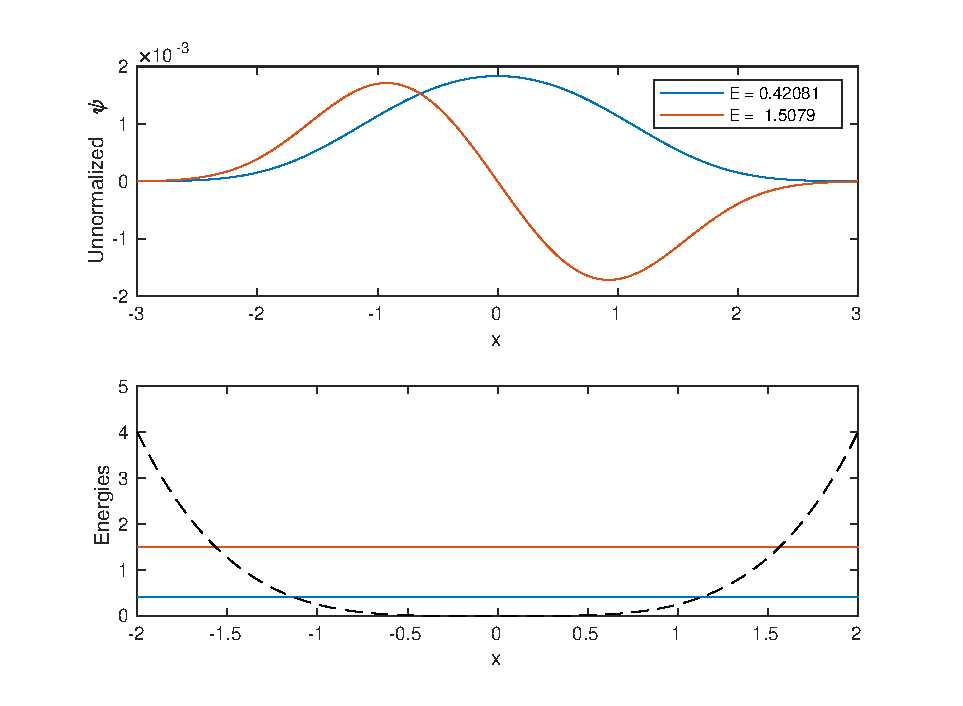
\includegraphics[width=0.75\textwidth]{problem3a.eps}
	\end{figure}



	
	MATLAB code:
	\begin{lstlisting}
	%%% Huan Q. Bui
	
	N = 1e6; % No. of points.
	hbar = 1;
	m = 1;
	x_start = -3;
	x_end = 3;
	x = linspace(x_start, x_end, N).'; % Generate column vector with N 
	dx = x(2) - x(1); % Coordinate step
	
	% Three-point finite-difference representation of Laplacian
	e = ones(N,1); % a column of ones
	Lap = spdiags([e -2*e e],[-1 0 1],N,N) / (dx^2);
	
	% potential
	U = x.^4/4;
	% Total Hamiltonian.
	H = -(1/2)*(hbar^2/m)*Lap + spdiags(U,0,N,N); % 0 indicates main diagonal 
	
	% Find lowest nmodes eigenvectors and eigenvalues of sparse matrix.
	nmodes = 2; 
	[V,E] = eigs(H,nmodes,'SM'); % find two smallest eigenvalues
	[E,ind] = sort(diag(E)); % convert E to vector and sort low to high.
	V = V(:,ind); % rearrange corresponding eigenvectors.
		
	% Generate plot of lowest energy eigenvectors V(x) and U(x).
	figure(1);
	subplot(2,1,1)
	plot(x, V);
	xlabel('x');
	ylabel('Unnormalized \psi');
	xlim([x_start x_end]);
	% Add legend showing Energy of plotted V(x).
	legendLabels = [repmat('E = ',nmodes,1), num2str(E)];
	legend(legendLabels)
	
	subplot(2,1,2)
	plot(x, (E(1))*ones(N,1),...
	x, (E(2))*ones(N,1), x, U, '--k');
	xlabel('x');
	ylabel('Energies');
	xlim([x_start/2 x_end/2]);
	\end{lstlisting}
	
	
	
	
	\textbf{\textcolor{blue}{Variational method:}} Alternatively, we could choose our guess solution for the ground state to be 
	\begin{align*}
	\psi_0(x,\al) = \Phi_0(x,\al)
	\end{align*}
	where $\al$ is a parameter and $\Phi_0(x,\al)$ is the ground state of the harmonic oscillator parameterized by $\al$ and is given by  
	\begin{align*}
	\Phi_0(x,\al) = \lp \f{\al}{\pi} \rp^{1/4} \exp\lp - \f{\al x^2}{2}  \rp
	\end{align*}
	The Rayleight-Ritz is given by 
	\begin{align*}
	E(\al) = \f{\int \psi \ham \psi\,dx}{\int \psi^2\,dx} = \int \psi \ham \psi\,dx = \f{3+4a^3}{16a^2} \implies \f{\p E}{\p \al} = -\f{3}{8a^3} + \f{1}{4} =0 \iff \al = \lp\f{3}{2}\rp^{1/3} 
	\end{align*}
	Upon checking this that $E(\al)$ obtains a minimum at $\al = $, we conclude that the ground state energy found using this naive variational method is 
	\begin{align*}
	\boxed{E_0 = \f{3+4(3/2)}{16(3/2)^{2/3}} \approx 0.429}
	\end{align*}
	which is consistent with what we found before. \\
	
	For the first excited state, we do the same thing except that we start from the first-excited wavefunction of the harmonic oscillator. 
	\begin{align*}
	\psi(x,\al) = \lp \f{\al}{\pi} \rp^{1/4}\sqrt{2 \al} x \exp\lp -\f{\al x^2}{2} \rp.
	\end{align*}
	Repeating the same procedure we find 
	\begin{align*}
	\boxed{E_1(\al) = \f{3(5+4a^3)}{16a^2} \implies E_1 \approx \min E(\al) =   1.527}
	\end{align*}
	which is again consistent with what we found by solving the SE numerically. 
	
	
	
	
	
	\item Ground and first excited energy for particle in the potential:
	\begin{align*}
	V(x) = -\f{1}{2}x^2 + \f{1}{24}x^4
	\end{align*}
	
	\textbf{\textcolor{blue}{Finite-difference method:}} Using the same 1D SE solver as before, we find that
	\begin{align*}
	\boxed{E_0 \approx 0.072} \quad\quad \boxed{E_1 \approx 0.452}
	\end{align*}
	
	Here is the graphical solution. 
	\begin{figure}[!htb]
		\centering
		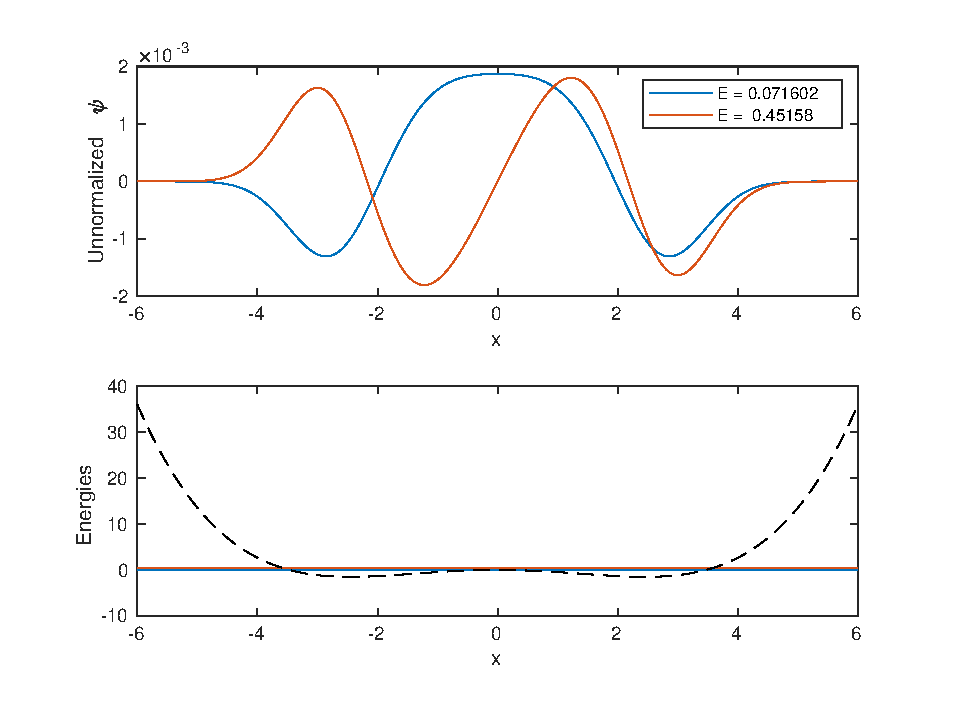
\includegraphics[width=0.75\textwidth]{problem3b.eps}
	\end{figure}
	
	
	The MATLAB code is identical to the MATLAB code in Part (a), except that the potential energy $V(x)$ is modified:
	\begin{lstlisting}
	% potential
	U = -x.^2/2 + x.^4/24;
	\end{lstlisting}
	
	
	
	
	
	\textbf{\textcolor{blue}{Shooting method:}} Searching for the ground state and first excited state energies via the shooting method we find with good accuracy:
	\begin{align*}
	\boxed{E_0 \approx 0.07160236} \quad\quad\quad \boxed{E_1 \approx 0.45157662}
	\end{align*} 
	
	Mathematica code:
	\begin{lstlisting}
	(*Double well potential*)
	v[x_] := -x^2/2 + x^4/24;
	xMax = 6;
	
	(*ground state energy*)
	energy = 0.07160236;
	solution = 
	NDSolve[{psi''[x] == -2 (energy - v[x]) psi[x], psi[-xMax] == 0, 
	psi'[-xMax] == 0.001}, psi, {x, -xMax, xMax}];
	
	Plot[psi[x] /. solution, {x, -xMax, xMax}]
	
	(*First excited state energy*)
	energy = 0.45157662;
	solution = 
	NDSolve[{psi''[x] == -2 (energy - v[x]) psi[x], psi[-xMax] == 0, 
	psi'[-xMax] == 0.001}, psi, {x, -xMax, xMax}];
	
	Plot[psi[x] /. solution, {x, -xMax, xMax}]
	\end{lstlisting}
	
	Shooting method output wavefunctions (up to overal phase factor compared to finite difference method):
	
	\begin{figure}[!htb]
		\centering
		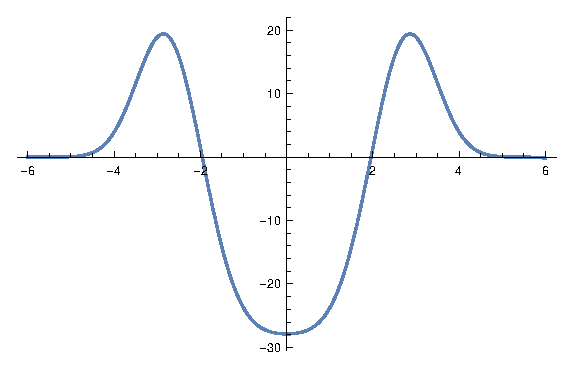
\includegraphics[width=0.35\textwidth]{problem3b1.eps}
		\caption{Ground state wavefunction}
	\end{figure}

	\begin{figure}[!htb]
		\centering
		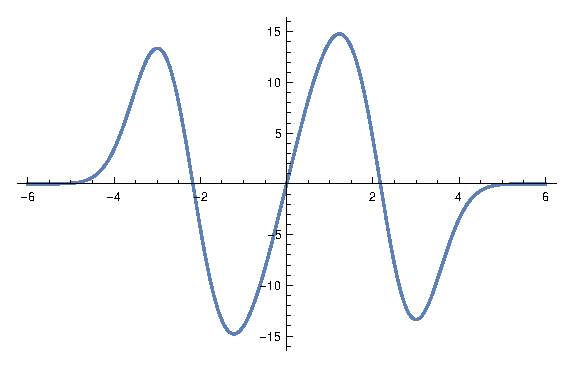
\includegraphics[width=0.35\textwidth]{problem3b2.eps}
		\caption{First excited state wavefunction}
	\end{figure}
	
	
	
	
	
	\item Ground state energy for particle in the potential:
	\begin{align*}
	W(x,y) = \f{1}{2}x^2 + \f{1}{2}y^2 - \sqrt{2}\abs{x-y}
	\end{align*}
	where we require that $\psi(x,y) = -\psi(y,x)$. \\
	
	
	\textbf{\textcolor{blue}{Finite difference method:}} I'm solving this problem in MATLAB, using the method of finite difference. To do this, I referenced \href{https://www.mathworks.com/matlabcentral/fileexchange/69885-q_schrodinger2d_demo}{{this page}} for a way to efficiently generate the 2D Laplacian operator. Once the Laplacian was setup, I had to test if my MATLAB code actually produces the correct energies for the usual 2D harmonic oscillator problem. And it did. Solving the 2D harmonic potential problem with $\omega = 1$ on a $100\times 100$ grid where $x,y\in [-4,4]$, I got the following energies for the lowest 4 eigenstates:
	\begin{lstlisting}
	Lowest energies requested: 
	0.9996
	1.9988
	1.9988
	2.9973
	\end{lstlisting}
	which are close to the correct values of $1,2,2,3$ (as there is a two-fold degeneracy in the first excited state). With this I proceeded to solve the problem for the modified potential:
	\begin{align*}
	W(x,y) = \f{1}{2}x^2 + \f{1}{2}y^2 - \sqrt{2}\abs{x-y}
	\end{align*}
	The caveat is that the lowest-energy solution to this problem is not what we want, since we also require that $\psi(x,y) = -\psi(y,x)$. This means that $\psi(x)$ must change sign under a reflection about the $y=x$ axis. To get to the correct solution, I had to go through the lowest-lying states and select the desired $\psi$ with the lowest energy. The result is the state with energy 
	\begin{align*}
	\boxed{E \approx 0.0320}
	\end{align*}
	We also notice that the discarded solutions have negative energies. 
	\begin{lstlisting}
	Lowest energies requested: 
	-0.1229
	-0.0127
	0.0320
	0.1291
	\end{lstlisting}
	
	The graphical solution is given below.
	
	\begin{figure}[!htb]
		\centering
		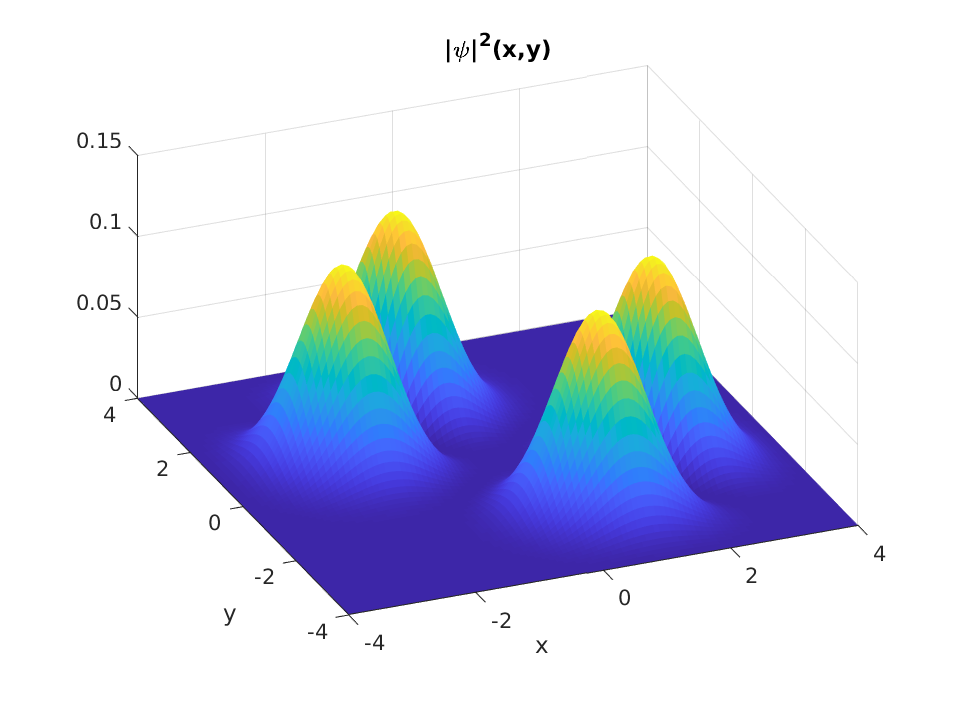
\includegraphics[width=0.55\textwidth]{problem3c1.eps}
		\caption{``Good'' ground state density function}
	\end{figure}
	
	\begin{figure}[!htb]
		\centering
		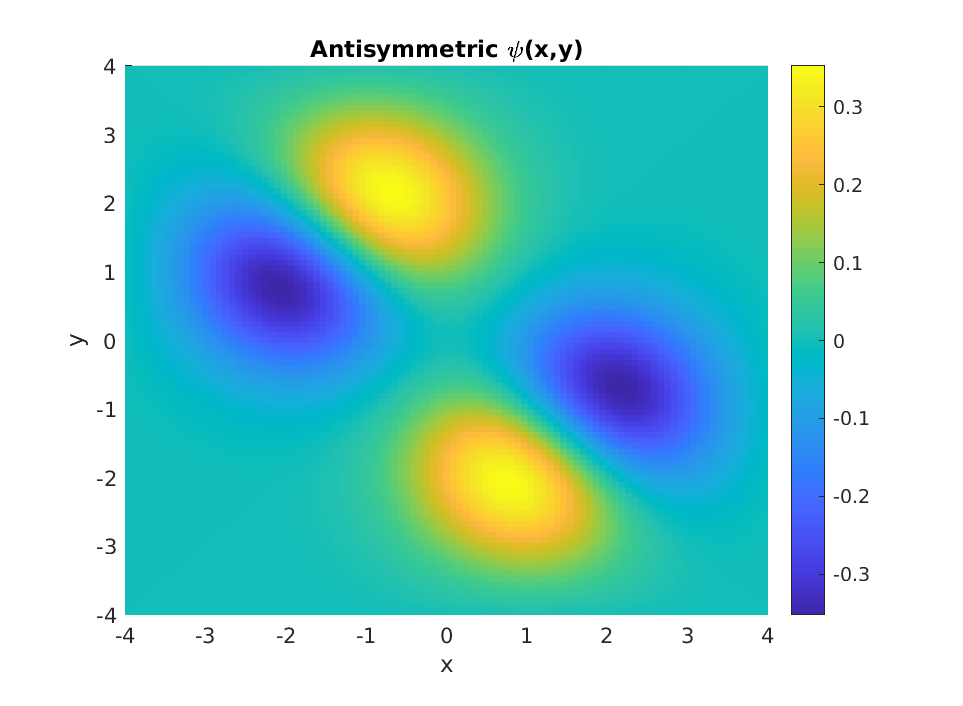
\includegraphics[width=0.55\textwidth]{problem3c2.eps}
		\caption{``Good'' ground state wavefunction}
	\end{figure}


	Full MATLAB code:
	\begin{lstlisting}
	hbar = 1;
	m = 1;
	
	N = 10^2;
	L = 4;
	
	x = linspace(-L,L,N);
	y = linspace(-L,L,N);
	
	dx= x(2) - x(1);
	dy= y(2) - y(1);
	
	%%% generate the 2D Laplacian operator quickly %%%
	%%% source:
	%%% https://www.mathworks.com/matlabcentral/fileexchange/69885-q_schrodinger2d_demo 
	
	Axy = ones(1,(N-1)*N);
	DX2 = (-2)*diag(ones(1,N*N)) + (1)*diag(Axy,-N) + (1)*diag(Axy,N);
	
	AA = ones(1,N*N);
	BB = ones(1,N*N-1);
	BB(N:N:end) = 0;
	DY2 =(-2)*diag(AA) + (1)*diag(BB,-1) + (1)*diag(BB,1);
	
	Lap = sparse(DX2/dx^2 + DY2/dy^2);
	
	% setting up potential
	[X,Y] = meshgrid(x,y);
	% harmonic potential 
	% U = X.^2/2 + Y.^2/2;
	% strange potential
	U = X.^2/2 + Y.^2/2 - sqrt(2)*abs(X-Y);
	
	% Total Hamiltonian.
	H = sparse(-(1/2)*(hbar^2/m)*Lap + diag(U(:))) ; 
	% Find lowest nmodes eigenvectors and eigenvalues of sparse matrix.
	nmodes = 4; 
	[Psi,E] = eigs(H,nmodes,'SM'); % find two smallest eigenvalues
	[E,ind] = sort(diag(E)); % convert E to vector and sort low to high.
	Psi = Psi(:,ind); % rearrange corresponding eigenvectors.

	% display all energies
	disp('Lowest energies requested: ')
	disp(E)
	
	%%%%%%%%%%%%%%%%%%%%%%% Normalization %%%%%%%%%%%%%%%%%%%%%%%%%
	for i=1:nmodes
	psi_temp = reshape(Psi(:,i),N,N);
	psi_result(:,:,i) = psi_temp / sqrt( trapz(y',trapz(x,abs(psi_temp).^2 ,2) , 1 ));  
	end
	
	%%% NOTE: want antisymmetric \psi, so pick eigenstate #3 to plot 
	
	% plot |psi|^2 for ground state only
	figure(1)
	surf(X,Y,abs(psi_result(:,:,3)).^2, 'LineWidth',0.1,'edgecolor','black', 'EdgeAlpha', 0.0 , 'FaceAlpha',1)
	title('|\psi|^2(x,y)')
	xlabel('x')
	ylabel('y')
	
	% plot \psi for ground state only
	figure(2)
	surf(X,Y,psi_result(:,:,3), 'LineWidth',0.1,'edgecolor','black', 'EdgeAlpha', 0.0 , 'FaceAlpha',1)
	view([0 0 90])
	colorbar;
	title('Antisymmetric \psi(x,y)')
	xlabel('x')
	ylabel('y')
	\end{lstlisting}
	
	\textbf{\textcolor{purple}{How would one do this problem variationally? I could imagine picking sines and cosines as basis functions, but setting up the solver and minimizing the Rayleigh-Ritz quotient seem very involved. Or maybe not... I haven't tried.}}
	
	
	
	
	\item \textbf{(Extra credit)} Ground state energy for particle in the potential:
	\begin{align*}
	V(x,y) = \f{1}{4}x^4 + \f{1}{6}y^6 + 2xy
	\end{align*}
	
	\textbf{Finite difference method:} I use the same approach for (c) to solve this problem. I simply modified the potential, and picked the lowest-energy state as the solution (since there's no symmetry requirement on $\psi$). The lowest energy is 
	\begin{align*}
	\boxed{E_0 \approx 0.359}
	\end{align*}
	MATLAB output for the 4 lowest energies:
	\begin{lstlisting}
	Lowest energies requested: 
	0.3859
	0.6345
	1.6811
	2.4703
	\end{lstlisting}
	
	The graphical solution is 
	\begin{figure}[!htb]
		\centering
		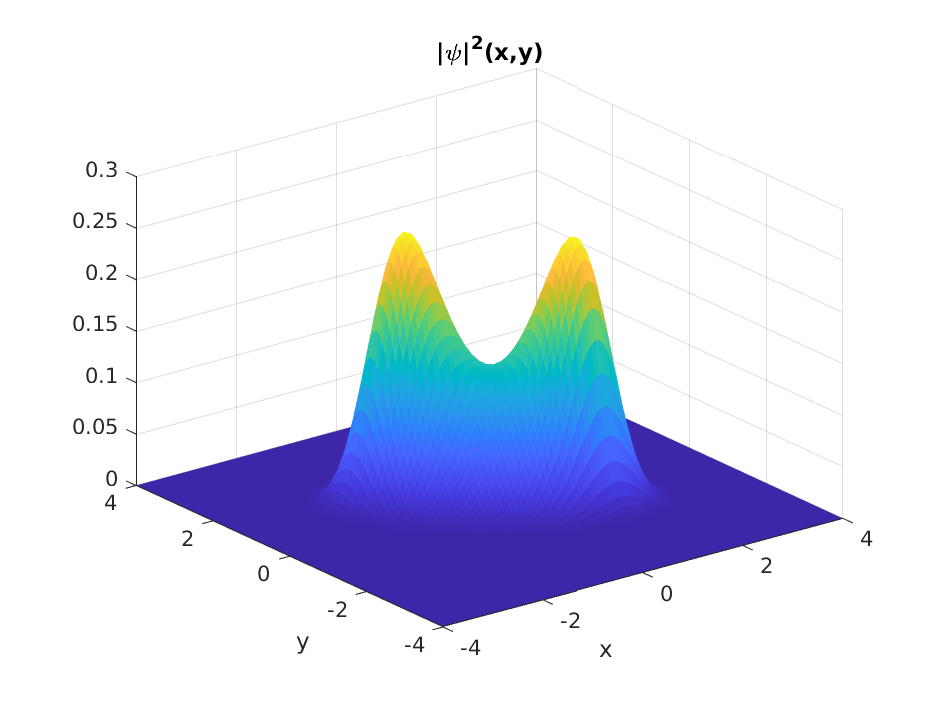
\includegraphics[width=0.55\textwidth]{problem3d1.eps}
		\caption{Ground state density function}
	\end{figure}
	
	\begin{figure}[!htb]
		\centering
		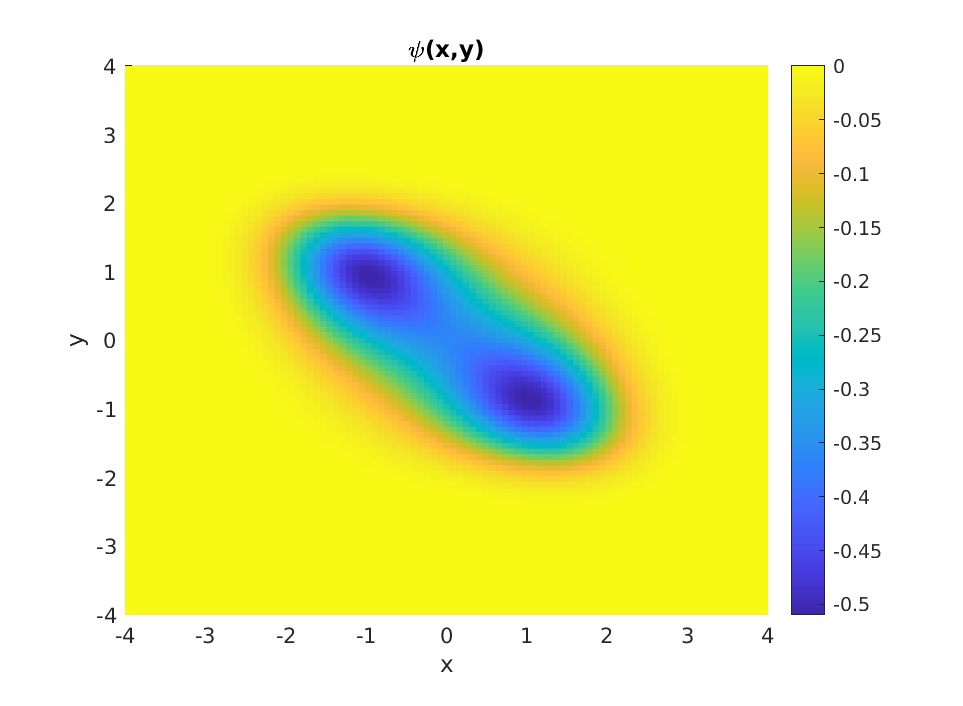
\includegraphics[width=0.55\textwidth]{problem3d2.eps}
		\caption{Ground state wavefunction}
	\end{figure}
	
	
	
\end{enumerate}

	
\end{document}








